% !TEX encoding = UTF-8
% !TEX program = pdflatex
% !TEX root = InformationRetrieval.tex
% !TEX spellcheck = it-IT

% 2 Dicembre 2016

\subsection{BM25}

La strada che ha portato ad ottenere il BM25 è stata molto lunga ed è iniziata negli anni 70.

\subsubsection{L'inizio del percorso}

Ripartendo dal BIM, la probabilità che un documento sia rilevante per una query può essere stimata con: 

\begin{align}
P(\rel | d,q) &\propto_q \frac{P(d|\rel, q)}{P(d| \notrel, q)} \\ 
&\approx \prod_{i \in V} \frac{P(TF_i=tf_i|rel,q)}{P(TF_i=tf_i | \notrel, q)} \underbrace{\frac{P(\rel|q)}{P(\notrel |q )}}_{\text{costante per tutti i documenti}} \nonumber  \\
&\approx \prod_{i \in V} \frac{P(TF_i = tf_i|\rel,q)}{P(TF_i=tf_i|\notrel,q)}\nonumber \\
&\approx \prod_{i \in q} \frac{P(TF_i = tf_i|\rel)}{P(TF_i=tf_i|\notrel)}
\end{align}

Da notare che la formula utilizza una variabile aleatoria diversa, per distinguere i passi che hanno portato al BM25 dalla formulazione del BIM. $TF_i$ è una variabile aleatoria che rappresenta la frequenza del termine $i$ all'interno del documento $d$. Il valore della frequenza per un dato termine è $tf_i$. $V$ continua invece ad essere il vocabolario.
Possono inoltre \textbf{limitare la produttoria} a tutti i termini delle query $i \in q$ e rimuovere il condizionamento, facendo l'ipotesi che tutti i termini che non compaiono nella query hanno la stessa probabilità di apparire sia nei rilevanti che non rilevanti. Quindi posso evitare di considerarli, perché il rapporto vale 1.

La produttoria non può essere calcolata perché lavora con numero troppo piccoli, quindi si considerano i logaritmi:

\begin{align}
P(\rel | d,q) &\propto_q \sum_q \underbrace{\log \Big(  \frac{P(TF_i=tf_i | \rel)}{P(TF_i=tf_i | \notrel )} \Big)}_{U_i(tf_i)} \\ 
&= \sum\limits_q U_i(tf_i) \\
&= \sum_{q,tf_i > 0} U_i(tf_i) + \sum_{q,tf_i = 0} U_i(0)
\end{align}

Nell'ultimo passaggio la sommatoria viene scomposta in modo da separare i termini con $tf_i > 0$ da quelli con $tf_i = 0$.

Nel procedimento del paper c'è un passaggio strano che l'autore l'ha motivato così: tutti i modelli prima del '74 partono dall'idea che ci sono le frequenze dei termini da sommare per calcolare lo score del documento, ma non viene mai presa in considerazione l'assenza dei termini.
Questo per motivi di efficienza perché nel '74 la potenza di calcolo era ridotta.

Quindi viene fatto il giochino di sommare e togliere la stessa quantità, in modo da poter raggruppare le sommatorie in un altro modo, per ottenere dei calcoli più semplici da fare.

\begin{align}
P(\rel | d,q) &\propto_q \sum_{q,tf_i > 0} U_i(tf_i) + \sum_{q,tf_i = 0} U_i(0) \nonumber \\
&= \sum_{q,tf_i > 0} U_i(tf_i) + \underbrace{\sum_{q,tf_i = 0} U_i(0) + \sum_{q, tf > 0} U(0)}_{\text{possono essere raggruppate}} - \sum_{q, tf > 0} U_i(0) \nonumber \\
&= \sum_{q, tf>0} \Big( U_i(tf_i) - U_i(0) \Big) + \underbrace{\sum_q U_i(0)}_{= 0}  \nonumber \\
&\propto_q \sum_{q, tf>0} \Big( U_i(tf_i) - \underbrace{U_i(0)}_{\text{costante per tutti i documenti}} \Big)
\end{align}

Quindi per calcolare la probabilità della rilevanza possono considerare solamente i termini che compaiono sia nella query che nei documenti.

Andando a espandere $U_i$ otteniamo:

\begin{align}
P(\rel | d,q) &\propto_q \sum_{q, tf>0} \Big( U_i(tf_i) - U_i(0) \Big) \nonumber \\
&\propto_q \sum_{q, tf>0} \log\frac{ P(TF_i = tf_i | \rel) P(TF_i = 0 | \notrel) }{P(TF_i = tf_i | \notrel) P(TF_i = 0 | \rel)} \label{eq:basic-prob}\\
&= \sum_{q, tf>0} W_i(tf_i)
\end{align}

Ottenendo così la formula basilare per andare a pesare la presenza di un termine della query all'interno di un documento, tenendo conto della frequenza con cui compare nel documento.

Dato che si tratta di un formulone, si può ridurre a:

\begin{align}
W_i(tf_i) &= \log\frac{ P(TF_i = tf_i | \rel) P(TF_i = 0 | \notrel) }{P(TF_i = tf_i | \notrel) P(TF_i = 0 | \rel)} = \log \frac{p_{tf_i} u_0}{u_{tf_i} p_0} \label{eq:basic-weight}
\end{align}

\noindent dove:

\begin{itemize}
\item $p_{tf_i} =  P(TF_i = tf_i | \rel) $ ovvero la probabilità che il termine $i$ \textbf{compaia} $tf_i$ volte nel documento, dato che il documento è \textbf{rilevante}.
\item $p_0 = P(TF_i = 0 | \rel) $ ovvero la probabilità che il termine $i$ \textbf{non compaia} nel documento, dato che il documento è \textbf{rilevante}.
\item $u_{tf_i} =  P(TF_i = tf_i | \notrel) $ ovvero la probabilità che il termine $i$ \textbf{compaia} $tf_i$ volte nel documento, dato che il documento è \textbf{non rilevante}.
\item $u_0 = P(TF_i = 0 | \notrel) $ ovvero la probabilità che il termine $i$ \textbf{non compaia} nel documento, dato che il documento è \textbf{non rilevante}.
\end{itemize}

Da notare che $p_0$ è diverso da $(1-p_{tf_i})$ perché $p_0$ modella l'assenza del termine e non il complemento di $p_{tf_i}$.

Nel caso di un modello con le variabili binarie, ovvero in cui $tf_i$ è 1 o 0, ci riconduciamo a qualcosa di simile al BIM, perché andando ad utilizzare i valori binari nell'equazione \ref{eq:basic-prob} otteniamo:

\begin{align}
P(\rel | d,q) &\propto_q \sum_{q, tf>0} \log\frac{ P(TF_i = 1 | \rel) P(TF_i = 0 | \notrel) }{P(TF_i = 1 | \notrel) P(TF_i = 0 | \rel)} \\
&= \sum_{q, tf>0} \log \Big(  \frac{p_i (1-\varphi_i)}{\varphi_i(1-p_i)} \Big)
\end{align}

Da notare che $\varphi_i$ è la $q_i$ del BIM, viene cambiato il simbolo per non fare confusione con la $q$ della query. 
Si ottiene quindi lo stesso risultato ottenuto dal modello binario utilizzando la teoria bayesiana.

\subsubsection{Il modello 2-Poisson}

Data una query ci sono termini che sono abbastanza infrequenti, che appaiono poche volte e termini che compaiono molto più frequentemente\footnote{Deriva da un'osservazione sperimentale}. Il tutto senza considerare le stop-word.

Si è osservato che la distribuzione di questi termini segue la distribuzione di Poisson:

$$
\mathcal{P}(\lambda) = \frac{\lambda^k}{k!}e^{-\lambda}
$$

Dove $k$ è un valore dato, che nel nostro caso rappresenta la frequenza del termine e $\lambda$ è un parametro della distribuzione. Il parametro $\lambda$ va ad influenzare la media della distribuzione.

La probabilità di una variabile aleatoria $X$ che segue la distribuzione di Poisson viene quindi calcolata con

$$
P(X = x) \frac{\lambda^x}{x!}e^{-\lambda}
$$

Viene quindi assunto che l'occorrenza dei termini sia casuale ma che si distribuisca attorno una certa media.

Da qui è nato il modello 1-Poisson, che calcola la probabilità che un termine $i$ appaia con una certa frequenza con

$$
P(TF_i = tf_i) \approx \frac{\hat{\lambda}^{tf_i}}{{tf_i}!}e^{-\hat{\lambda}}
$$

\noindent dove $\hat{\lambda} = \cfrac{c_i}{N}$, ovvero $\lambda$ viene stimato utilizzando la frequenza media del termine $i$ all'interno della collezione ($c_i$ è la collection frequency del termine e $N$ è il numero di documenti presenti nella collezione).
Questo però non andava benissimo e quindi si è passati al 2-Poisson model.

Si è osservato che i termini possono essere divisi in due gruppi: un gruppo che contiene i termini che appaiono poche volte $\mu$ (e che seguono una distribuzione con $\lambda = \mu \approx 1$) e l'altro che contiene quelli che compaiono molte volte $\lambda > \mu$. 

L'ipotesi che è stata fatta è che la probabilità di osservare un termine generico in un documento è data da una "\textit{mistura}" di queste due distribuzioni. Ovvero preso un documento a caso, la probabilità di osservare un termine dipende dalle due distribuzioni $\mu$ e $\lambda$.

C'è poi il concetto di \textbf{éliteness}, fissato un termine all'interno di un documento, tanto più frequente sarà quel termine, tanto più d'élite sarà quel documento per il concetto rappresentato dal termine. 
Quindi, tanto più frequente è un termine all'interno del documento, tanto più il documento è d'élite rispetto al concetto descritto dal termine e di conseguenza, se il termine compare anche nella query, la probabilità che il documento sia anche rilevante aumenta.

Il modello 2-Poisson si basa quindi su due distribuzioni, che modellano la probabilità che un termine che appare con una certa frequenza nel documento sia d'élite o meno:

\begin{align}
a_{tf} &= P(TF_i = tf_i | E_i = \elite) = \frac{\lambda^{tf_i}}{{tf_i}!}e^{-\lambda}\\
n_{tf} &= P(TF_i = tf_i | E_i = \notelite) = \frac{\mu^{tf_i}}{{tf_i}!}e^{-\mu}
\end{align}

La distribuzione di un termine in un documento segue dipende quindi da entrambe le distribuzioni, perché non si sa se quel termine è d'élite nel documento o meno, ovvero:

$$
P(TF_i = tf_i) = \pi \frac{\lambda^{tf_i}}{{tf_i}!}e^{-{\lambda}} + (1 - \pi) \frac{\mu^{tf_i}}{{tf_i}!}e^{-\mu}
$$

\noindent dove $\pi$ è la probabilità che il documento sia d'élite e tipicamente non è nota.

Il tutto per dire che per pesare un termine bisogna tenere in considerazione sia la rilevanza del documento che l'éliteness ed entrambe le caratteristiche sono influenzate dalla frequenza del termine. 

Inoltre, dato che l'éliteness e la rilevanza sono due cose distinte, ci possono essere dei documenti d'élite per un certo argomento ma che non sono rilevanti per la query.
Si ha poi che un documento è d'élite per un determinato termine se questo termine è molto presente, senza prendere in considerazione la rilevanza.
Quindi:

\begin{align}
P(TF_i = tf_i | \rel) &= P(tf_i | E_i = \elite)P(E_i = \elite | \rel) + P(tf_i |E_i = \notelite)P(E = \notelite | \rel) \\
P(TF_i = tf_i | \notrel) &= P(tf_i | E_i = \elite)P(E_i = \elite | \notrel) + P(tf_i |E_i = \notelite)P(E_i = \notelite | \notrel) 
\end{align}

Si può quindi abbreviare con

\begin{itemize}
	\item $p_i' = P(E_i = \elite | \rel)$
	\item $q_i' = P(E_i = \elite | \notrel)$
\end{itemize}

e andare a pesare il termine con la formula \ref{eq:basic-weight}, sostituendo le due formule sopra riportate:

\begin{align}
W_i(tf_i) &=  \log\frac{ P(TF_i = tf_i | \rel) P(TF_i = 0 | \notrel) }{P(TF_i = tf_i | \notrel) P(TF_i = 0 | \rel)} \\
&= \log \frac{
\big(p_i'\lambda^{tf_i}e^{-\lambda} + (1-p_i')\mu^{tf_i}e^{-\mu}\big)\big(q_i'e^{-\lambda} + (1-q_i')e^{-\mu}\big)
}{
\big(q_i'\lambda^{tf_i}e^{-\lambda} + (1-q_i')\mu^{tf_i}e^{-\mu}\big)\big(p_i'e^{-\lambda} + (1-p_i')e^{-\mu}\big)
} \label{eq:wtf}
\end{align}


C'è quindi il problema della stima di questi 4 parametri, nessuno dei quali può essere stimato osservando i documenti a disposizione, perché l'éliteness è una variabile nascosta. \`E stata questa la critica degli autori del BM25 verso il 2-Poisson. Tuttavia le osservazioni alla base di questo modello si sono rivelate essere corrette.


\subsubsection{Approssimazioni del 2-Poisson}

Risulta quindi necessario utilizzare un'approssimazione della funzione di peso del 2-Poisson.
Per fare questa approssimazione si può osservare che:

\begin{enumerate}
	\item Se $tf_i = 0$, anche $W_i(0) = 0$.
	\item La funzione cresce in monotonicamente come $tf_i$.
	\item C'è un massimo asintotico.
	\item Il massimo è simile al sistema di pesi del BIM:
	$$
	\lim\limits_{tf_i \to \infty} W_i^{elite}(tf_i) = \log \frac{p_i'(1-q_i')}{q_i'(1-p_i')}
	$$
\end{enumerate}

\begin{figure}[htbp]
	\centering
	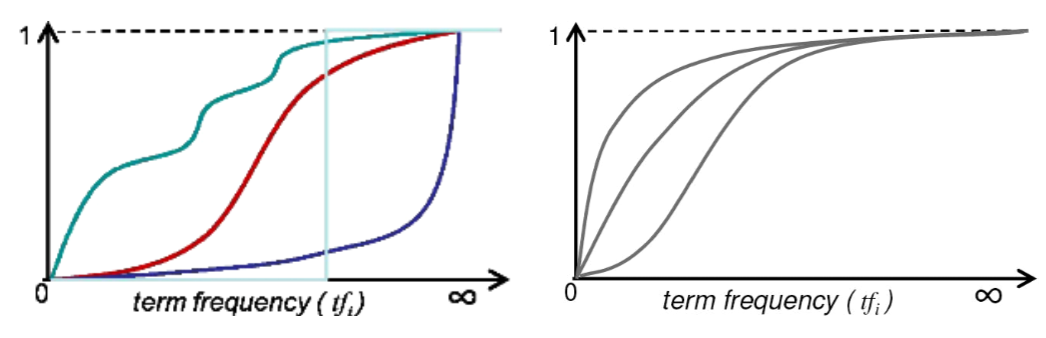
\includegraphics[width=0.9\textwidth]{images/l19-fig-1.png}
	\caption{A sinistra: alcune possibile funzioni di saturazione che sono compatibili con i 4 punti dell'elenco. A destra: funzioni di saturazione generate dal 2-Poisson.}
\end{figure}

Quindi se l'éliteness fosse osservabile, sarebbe possibile trattarla come un attributo binario e utilizzare la stessa funzione di pesatura del BIM.
Questo a livello asintotico ha senso. Perché dato che l'unica associazione tra $tf_i$ e la rilevanza passa attraverso l'éliteness, la miglior informazione che possiamo sperare di ottenere da un termine è che il documento è d'élite per quel termine. In realtà la nostra informazione riguardo questo score è probabilistica, e quindi il peso del termine viene ridotto secondo la questa probabilità. Questo comportamento prende il nome di \textbf{saturazione}.
Da notare che l'unico caso in cui non vale la saturazione è quando la rilevanza e l'éliteness coincidono, ottenendo un limite infinito e rendendo il peso del termine lineare rispetto alla frequenza, come avviene con $tf\cdot idf$.

Gli autori di BM25 hanno quindi deciso di approssimare l'effetto dell'éliteness utilizzando la curva

\begin{align}
\frac{tf_i}{k + tf_i} \label{eq:raw}
\end{align}

\noindent per qualche $k > 0$.

L'approssimazione utilizzata inizialmente per l'equazione \ref{eq:wtf} è quindi

\begin{align*}
W_i(tf_i) &= \frac{tf_i}{k + tf_i}  w_i^{RSJ} \\
&=\frac{tf_i}{k + tf_i}  \log \bigg( \frac{N_{t_iR} + 0.5}{N_R - N_{t_iR} + 0.5} \frac{N - N_R - N_{t_i} + N_{tR + 0.5}}{N_{t_i} + N_{t_iR} +0.5} \bigg)
\end{align*}

\noindent dove $w_i^{RSJ}$ deriva dall'equazione \ref{eq:wrsj} ed è una versione semplificata del BM15.

Tutto questo funziona se assumiamo che i documenti hanno la stessa lunghezza perché consideriamo quante volte compare un termine all'interno di un documento, senza preoccuparci del numero totale di termini. Ovviamente non possiamo fare tale assunzione.

I primi modelli che tenevano in considerazione la lunghezza del documento, modificavano la frequenza del termine dividendola per la lunghezza del documento $dl$, effettuando una normalizzazione della frequenza.

$$
dl = \sum\limits_{i \in V} tf_i
$$

\noindent Si è quindi ottenuto un BM-qualcosa.

$$
W_i(tf_i) = \frac{\cfrac{tf_i}{dl}}{k + \cfrac{tf_i}{dl}}  w_i^{RSJ}
$$

Infine nel '96 sono stati accorpati il BM11 e BM15 si è ottenuto il BM25. Ci sono arrivati osservando che i documenti più corti avevano una maggior probabilità di essere recuperati. 
Hanno quindi scelto di bilanciare l'effetto della lunghezza aumentando leggermente la probabilità di recuperare un documento più lungo della media e diminuendo la probabilità per quelli sotto la media.

Questo è stato fatto andando a normalizzare la $tf_i$ con

$$
B = (1-b)+ b\frac{dl}{avgdl}
$$

\noindent dove $avgdl$ è la lunghezza media dei documenti della collezione.
Quindi se $b=1$ viene fatta la normalizzazione completa, dando maggiore probabilità di retrieval ai documenti corti mentre se $b=0$ viene data maggiore probabilità di retrieval ai documenti lunghi, in quanto non viene fatta la normalizzazione.

\begin{figure}[htbp]
	\centering
	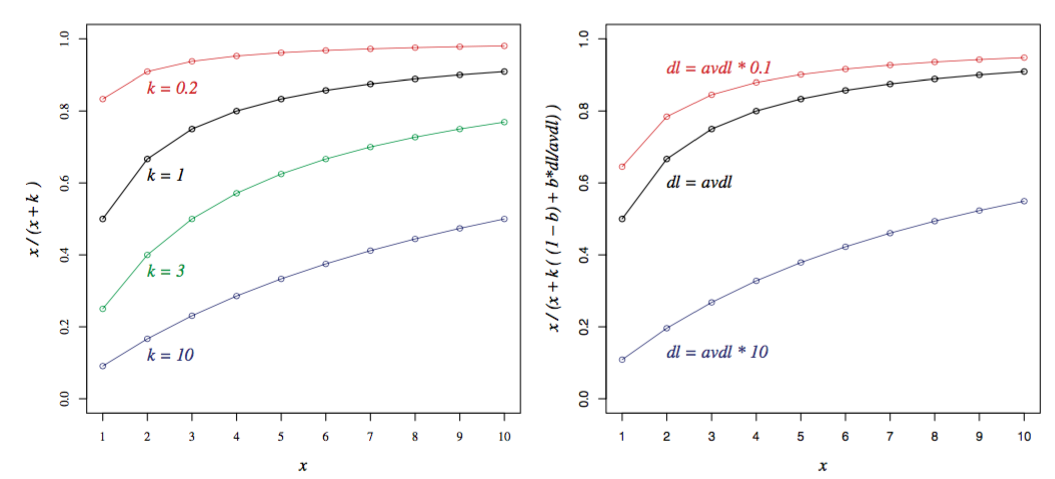
\includegraphics[width=0.9\textwidth]{images/l19-fig-2.png}
	\caption{A sinistra: funzioni di saturazione generate con l'equazione \ref{eq:raw}. A destra: funzioni di saturazione generate normalizzando $tf_i$ con $B$ ($k=1, b=0.5$).}
\end{figure}


Mettendo tutto assieme si ottiene il BM25 semplificato: 

\begin{align}
\boxed{
	W_i^{BM25}(tf_i) = \frac{tf_i}{k_1\bigg((1-b)+ b\cfrac{dl}{avgdl}\bigg) + tf_i } w_i^{RSJ}
}
\end{align}

Tipicamente come parametri viene utilizzato $k_1=1.5$ e $b=0.75$, tuttavia possono essere ottimizzati ad hoc in modo sperimentale.
Questo modello avrebbe un'ulteriore componente che tiene conto della frequenza dei termini della query. Tale fattore viene però tenuto tipicamente uguale a 1, perché la frequenza dei termini nella query è sempre 1, salvo i rari casi in cui la query è rappresentata da un documento.
C'è poi un'altra variante che sostituisce moltiplica il numeratore per $k_1+1$.

La versione "completa" del BM25 è quindi:

\begin{align}
W_i^{BM25}(tf_i) = \frac{(k_1+1)tf_i}{k_1\bigg((1-b)+ b\cfrac{dl}{avgdl}\bigg) + tf_i } \times \frac{(k_3+1)qtf_i}{k_3 + qtf_i} \times w_i^{RSJ}
\end{align}

\noindent Da notare che manca il termine $k_2$, questo perché era un parametro del modello che è stato rimosso in quanto tutti gli esperimenti che sono stati fatti hanno provato che i risultati migliori si trovano con $k_2=0$ e quindi non viene più considerato.

\begin{itemize}
\item non posso chiedervi di  calcolare delle formule con bm25

\item posso chiedervi che data, una collezione di documenti con tf e rilevanza, calcolare qual'è il documento più rilevante (calcolo di log p/q (1-q)/(1-p), con numeri appropriati in modo che non serva la calcolatrice.

\item posso chiedervi le ipotesi di partenza da 2-poisson a bm25. Interessa il ragionamento. Dato il formulone generale, quali sono le ipotesi semplificative che permettono di arrivare a bm25.
\end{itemize}










